%------------------------------------------------------------------------------------------------------------
\section{Database management} \label{sec:DataBases}
%------------------------------------------------------------------------------------------------------------

This section covers the description of databases that will be used later by AMIDST learning and inference algorithms implemented in the toolbox.  Figure~\ref{fig:DataBase} shows a high-level overview of the key components of the AMIDST toolbox. It illustrates mainly the different database functionalities and how they are connected to the core component \comp{PGM} through both the \comp{Learning Engine} and \comp{Inference Engine} components. In what follows, we describe each of the database functionalities, along with a code excerpt containing a brief example, then we introduce briefly the \comp{Learning Engine} and \comp{Inference Engine} that will be presented in more details in Deliverable 3.2.

\vspace{-0.4in}
  \begin{figure}[ht!]
    \centering
    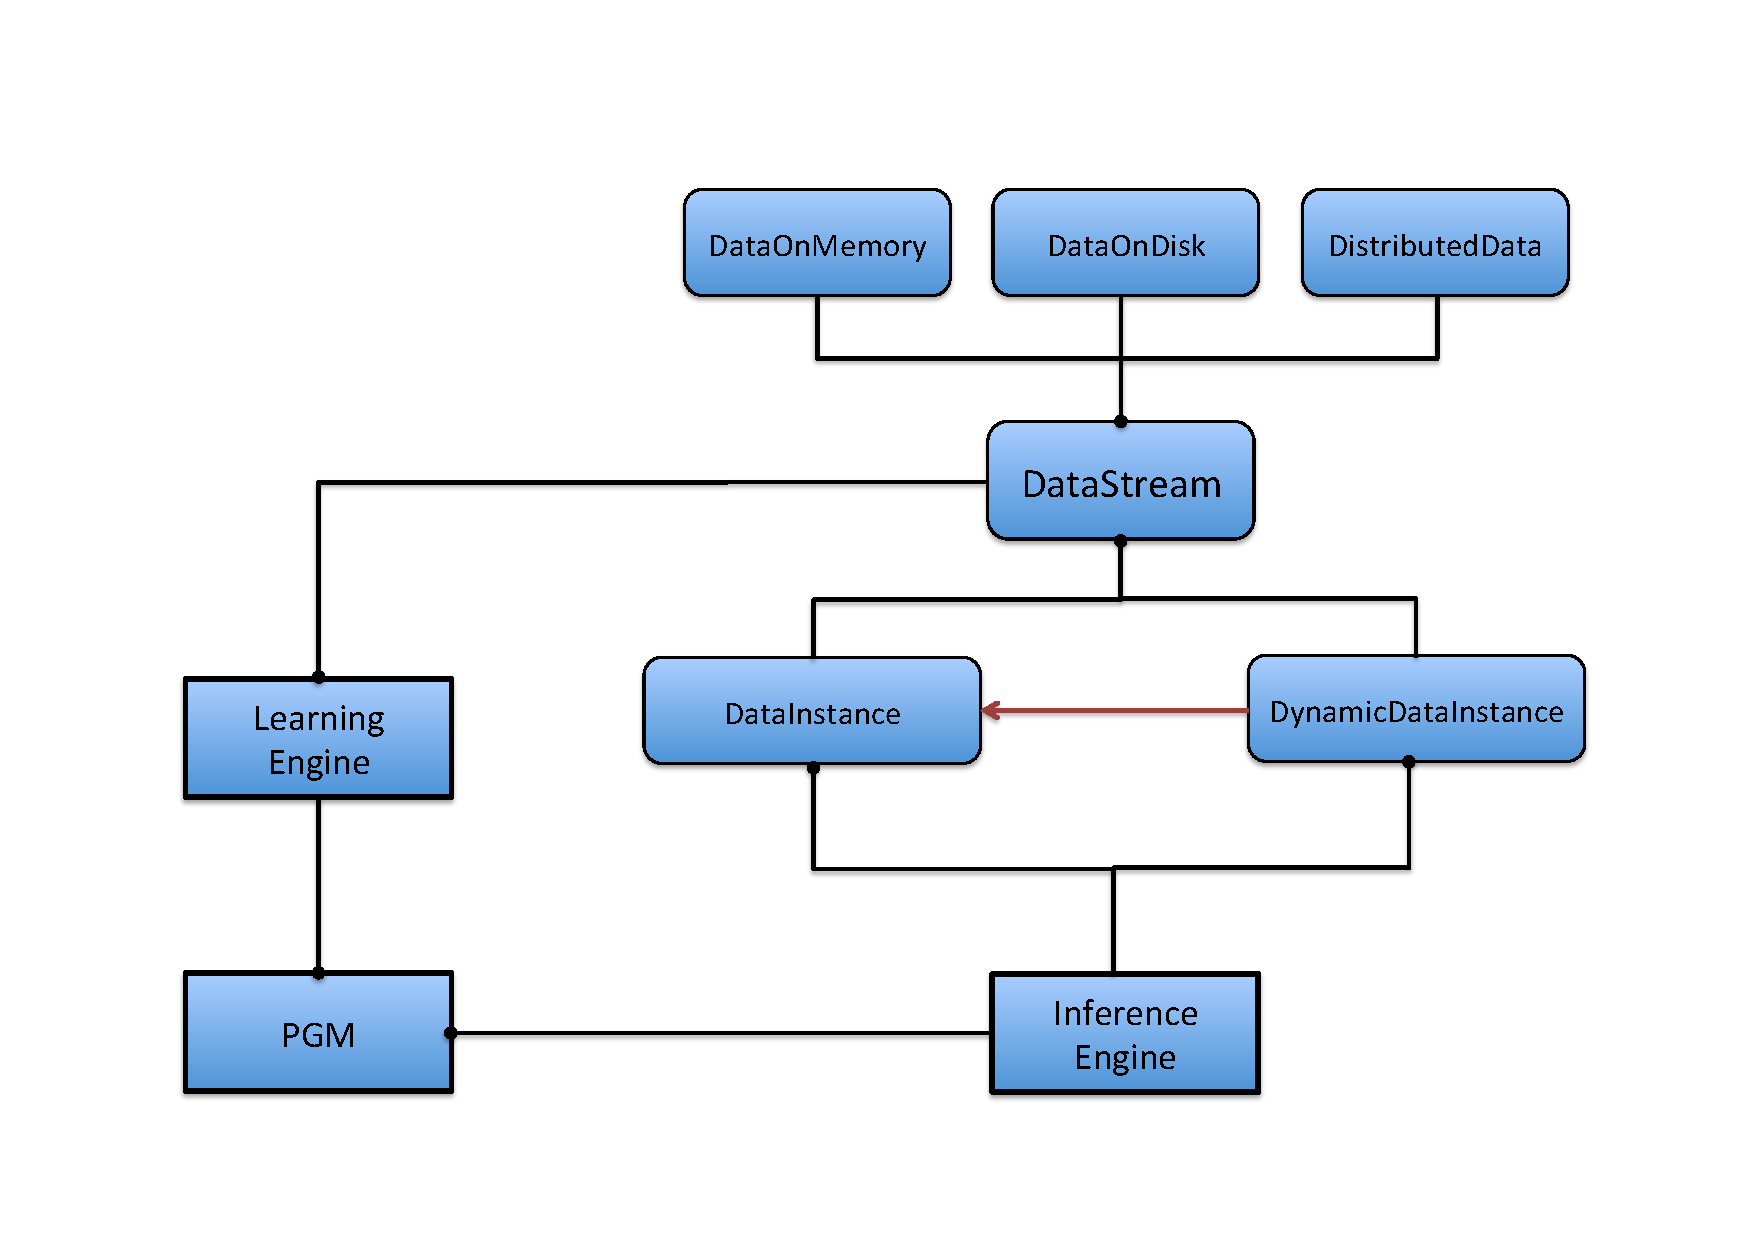
\includegraphics[width=\linewidth]{./figures/DataBase}
    \vspace{-0.8in}
    \caption{Illustration of the main database management functionalities and their connection with PGM, learning engine, and inference engine components. }
    \label{fig:DataBase}
  \end{figure}
 
%------------------------------------------------------------------------------------------------------------
\subsection{DataStream}
%------------------------------------------------------------------------------------------------------------   

In the AMIDST framework, we consider a \comp{DataStream} as a data source, i.e., a streaming data where records arrive at high frequency with no storage of historical data in memory. \comp{DataStream} is connected to either \comp{DataInstance} and \comp{DynamicDataInstance} components. 

The employed design is intended to support future users and developers of the AMIDST toolbox in the potential design and implementation of other database specifications; the only restriction being that new database components should implement the interface defined by the \comp{DataStream} component. 

%------------------------------------------------------------------------------------------------------------
\subsection{DataInstance}
%------------------------------------------------------------------------------------------------------------  
  
The \comp{DataInstance} component consists of a single class that represents a particular evidence configuration, such as the observed values of a collection of variables in a particular data row. 


\vspace{-0.1in}
\begin{table}[H]
\begin{tabular}{l} \\ \hline
                \texttt{DataStream<DataInstance> data = }\\
                 \texttt{~~~~~~~~~~DataStreamLoader.loadFromFile("datasets/staticData.arff");}\\\hline 
\end{tabular}
\end{table}

%------------------------------------------------------------------------------------------------------------
\subsection{DynamicDataInstance}
%------------------------------------------------------------------------------------------------------------  

The \comp{DynamicDataInstance} component consists of two data rows, such that the first refers to the past while the second refers to the present. In addition to the attributes present in each data row, \comp{DynamicDataInstance} could be characterised also with a TimeID and a SequenceID stored as additional attributes in the considered dynamic data.

\vspace{-0.1in}
\begin{table}[H]
\begin{tabular}{l} \\ \hline
        \texttt{DataStream<DynamicDataInstance> data = }\\
        \texttt{~~~~ DynamicDataStreamLoader.loadFromFile("datasets/dynamicData.arff");}\\\hline 
\end{tabular}
\end{table}


%------------------------------------------------------------------------------------------------------------
\subsection{Learning Engine}
%------------------------------------------------------------------------------------------------------------  

The \comp{Learning Engine} component consists of the implementations of the different learning algorithms for static and dynamic BNs, ensuring both structural and parameter learning. For structural learning, the AMIDST toolbox currently supports standard PC and parallel TAN algorithms by interfacing to the Hugin API (cf.\ Task 4.1). For parameter learning, a fully Bayesian approach is pursued in the AMIDST framework (cf.\ Task 4.2 and Task 4.4), which means that parameter learning reduces to the task of inference for which two approaches will be considered:, namely, variational message passing and expectation propagation. 

More implementation details about these algorithms will be provided in Deliverable 3.2. Note also that the design of the \comp{Learning Engine} is flexible in the sense that it easily accommodates potential future learning-based extensions, such as Bayesian learning based on importance sampling or maximum likelihood learning using the expectation maximization algorithm (see Section 3 in Deliverable 4.1 \cite{Deliverable4.1}). 
 
%------------------------------------------------------------------------------------------------------------
\subsection{Inference Engine}
%------------------------------------------------------------------------------------------------------------  

The \comp{Inference Engine} component consists of the implementations of both variational message passing and expectation propagation algorithms 
for probabilistic graphical models with conjugate-exponential distribution families (see Section 3, Deliverable 4.1 \cite{Deliverable4.1}). 

The different functionalities of the \comp{Inference Engine} component are ensured in AMIDST toolbox through tailored exponential family implementations of the standard distributions that are part of the AMIDST framework (such as the conditional linear Gaussian distributions). More details about this component will be provided in Deliverable 3.2.  